%%%%%%%%%%%%%%%%%%%%%%%%%%%%%%%%%%%%%%%%%
% Beamer Presentation
% LaTeX Template
% Version 1.0 (10/11/12)
%
% This template has been downloaded from:
% http://www.LaTeXTemplates.com
%
% License:
% CC BY-NC-SA 3.0 (http://creativecommons.org/licenses/by-nc-sa/3.0/)
%
%%%%%%%%%%%%%%%%%%%%%%%%%%%%%%%%%%%%%%%%%

%----------------------------------------------------------------------------------------
%	PACKAGES AND THEMES
%----------------------------------------------------------------------------------------

\documentclass{beamer}
\usepackage{xeCJK}
\usepackage{times}
\usepackage{multirow}
\usepackage{diagbox}
\usepackage{subfigure}

\newcommand{\cccve}{CCC\{$v_\mathrm{e}$\}}
\newcommand{\ccckt}{CCC\{$K^\mathrm{trans}$\}}
\newcommand{\kt}{$K^\mathrm{trans}$}
\newcommand{\Ve}{$v_\mathrm{e}$}

\setCJKfamilyfont{song}{SimSun}                             %宋体 song
\newcommand{\song}{\CJKfamily{song}} 

\mode<presentation> {

% The Beamer class comes with a number of default slide themes
% which change the colors and layouts of slides. Below this is a list
% of all the themes, uncomment each in turn to see what they look like.

%\usetheme{default}
%\usetheme{AnnArbor}
%\usetheme{Antibes}
%\usetheme{Bergen}
%\usetheme{Berkeley}
%\usetheme{Berlin}
%\usetheme{Boadilla}
%\usetheme{CambridgeUS}
%\usetheme{Copenhagen}
%\usetheme{Darmstadt}
%\usetheme{Dresden}
%\usetheme{Frankfurt}
%\usetheme{Goettingen}
%\usetheme{Hannover}
%\usetheme{Ilmenau}
%\usetheme{JuanLesPins}
%\usetheme{Luebeck}
%\usetheme{Madrid}
%\usetheme{Malmoe}
%\usetheme{Marburg}
%\usetheme{Montpellier}
%\usetheme{PaloAlto}
%\usetheme{Pittsburgh}
%\usetheme{Rochester}
%\usetheme{Singapore}
%\usetheme{Szeged}
\usetheme{Warsaw}

% As well as themes, the Beamer class has a number of color themes
% for any slide theme. Uncomment each of these in turn to see how it
% changes the colors of your current slide theme.

%\usecolortheme{albatross}
%\usecolortheme{beaver}
%\usecolortheme{beetle}
%\usecolortheme{crane}
%\usecolortheme{dolphin}
%\usecolortheme{dove}
%\usecolortheme{fly}
%\usecolortheme{lily}
%\usecolortheme{orchid}
%\usecolortheme{rose}
%\usecolortheme{seagull}
%\usecolortheme{seahorse}
%\usecolortheme{whale}
%\usecolortheme{wolverine}

%\setbeamertemplate{footline} % To remove the footer line in all slides uncomment this line
%\setbeamertemplate{footline}[page number] % To replace the footer line in all slides with a simple slide count uncomment this line

%\setbeamertemplate{navigation symbols}{} % To remove the navigation symbols from the bottom of all slides uncomment this line
}

\usepackage{graphicx} % Allows including images
\usepackage{booktabs} % Allows the use of \toprule, \midrule and \bottomrule in tables
\newcommand{\argmin}{\operatornamewithlimits{arg\ min~}}

%----------------------------------------------------------------------------------------
%	TITLE PAGE
%----------------------------------------------------------------------------------------

\title[博士学位论文答辩]{基于压缩感知的DCE-MRI重建与基于GPU的MRF字典生成和匹配} % The short title appears at the bottom of every slide, the full title is only on the title page

\author[王冬]{
答辩人:王冬 \\
指导教师:杨孝平\quad 教授
} % Your name
\institute[南京理工大学] % Your institution as it will appear on the bottom of every slide, may be shorthand to save space
{
南京理工大学 \\ % Your institution for the title page
\medskip
\textit{理学院} 
}
\date{2019年6月11日} % Date, can be changed to a custom date

\begin{document}

\begin{frame}
\titlepage % Print the title page as the first slide
\end{frame}

\begin{frame}
\frametitle{目录} % Table of contents slide, comment this block out to remove it
\tableofcontents % Throughout your presentation, if you choose to use \section{} and \subsection{} commands, these will automatically be printed on this slide as an overview of your presentation
\end{frame}

%----------------------------------------------------------------------------------------
%	PRESENTATION SLIDES
%----------------------------------------------------------------------------------------

%------------------------------------------------
\section{引言}
%------------------------------------------------
\AtBeginSection[]
{
    \begin{frame}
        \tableofcontents[currentsection,hideallsubsections]
    \end{frame}
}

\subsection{研究背景}
\begin{frame}
	\frametitle{研究背景--压缩感知MR重建}
	\begin{itemize}
		\item 基于压缩感知的MR重建是近十几年研究的热点。
		\item 压缩感知理论表明,可以从少量k-space数据中通过算法精确地重建出MR图像
		\item MRI成像速度慢,而压缩感知可以加速MR成像,因此在临床和研究上都有着重要的意义。
	\end{itemize}
\end{frame}

\begin{frame}
	\frametitle{研究背景--压缩感知MR重建}
	基于压缩感知的MR重建模型:
	\begin{equation}
		\min_X \frac{1}{2}\|AX-B\|_F^2+\alpha\|TX\|_1
	\end{equation}
	其中$X$为待重建的MR图像,$B$为采样收集到k-space数据,$T$为某个稀疏变换。
	
	这里$A=M\cdot\mathcal{F}$为采样矩阵,其中$\mathcal{F}$为傅里叶变换,$M$为采样模式。
\end{frame}

\begin{frame}
	\frametitle{研究背景--压缩感知MR重建}
	\begin{itemize}
		\item 常用的稀疏项:傅里叶变换、小波变换、TV/TGV、核范数、字典学习、深度神经网络 ...
		\item 常用的采样方式:Cartesian、伪径向/径向、螺旋 ...
		\item 常用的重建算法:ADMM、FISTA、Primal-Dual ...
	\end{itemize}
\end{frame}


\begin{frame}
	\frametitle{研究背景--压缩感知MR重建}
	压缩感知MR重建存在的问题:
	\begin{itemize}
		\item 对于胸部DCE-MRI(磁共振动态对比增强),其稀疏项不确定,尤其是时间方向上的稀疏项
		\item 使用TV作为正则项重建出的MR图像存在阶梯效应,边界不清的问题
		\item 动态MR图像的时间分辨率与空间分辨率之间权衡
		\item ...
	\end{itemize}
\end{frame}

\begin{frame}
	\frametitle{研究背景--MRF}
	\begin{itemize}
		\item 磁共振指纹(MRF)是一种新的定量MRI方法
		\item 可以在单次数据采集中同时获取多个组织参数,如$T_1$,$T_2$和质子密度
		\item 这些参数可以为医生提供更加客观的标准,增加诊断的精度
	\end{itemize}
\end{frame}

\begin{frame}
\frametitle{研究背景--MRF}
	MRF重建参数图的过程中涉及到三个步骤,分别为信号采集、预定义字典生成和模板匹配。
	\begin{itemize}
		\item 选取对所需参数敏感的MR序列对信号进行采样,并且序列的参数,如重复时间($T_R$)等,需要随着时间随机变动,使得不同参数的组织在MR序列中产生独特的信号演化(指纹) -- bSSFP/uSSFP ...
		\item 字典中包含着不同参数的组织在该MR序列中的模拟演化 -- EPG/Bloch ...
		\item 模式识别算法用来比较每个体素指纹和字典中元素的匹配度,重建参数图 -- 模板匹配、降维(SVD/grouping)、深度神经网络 ...
	\end{itemize}
\end{frame}


\begin{frame}
\frametitle{研究背景--MRF}
	\begin{figure}
		\centering
		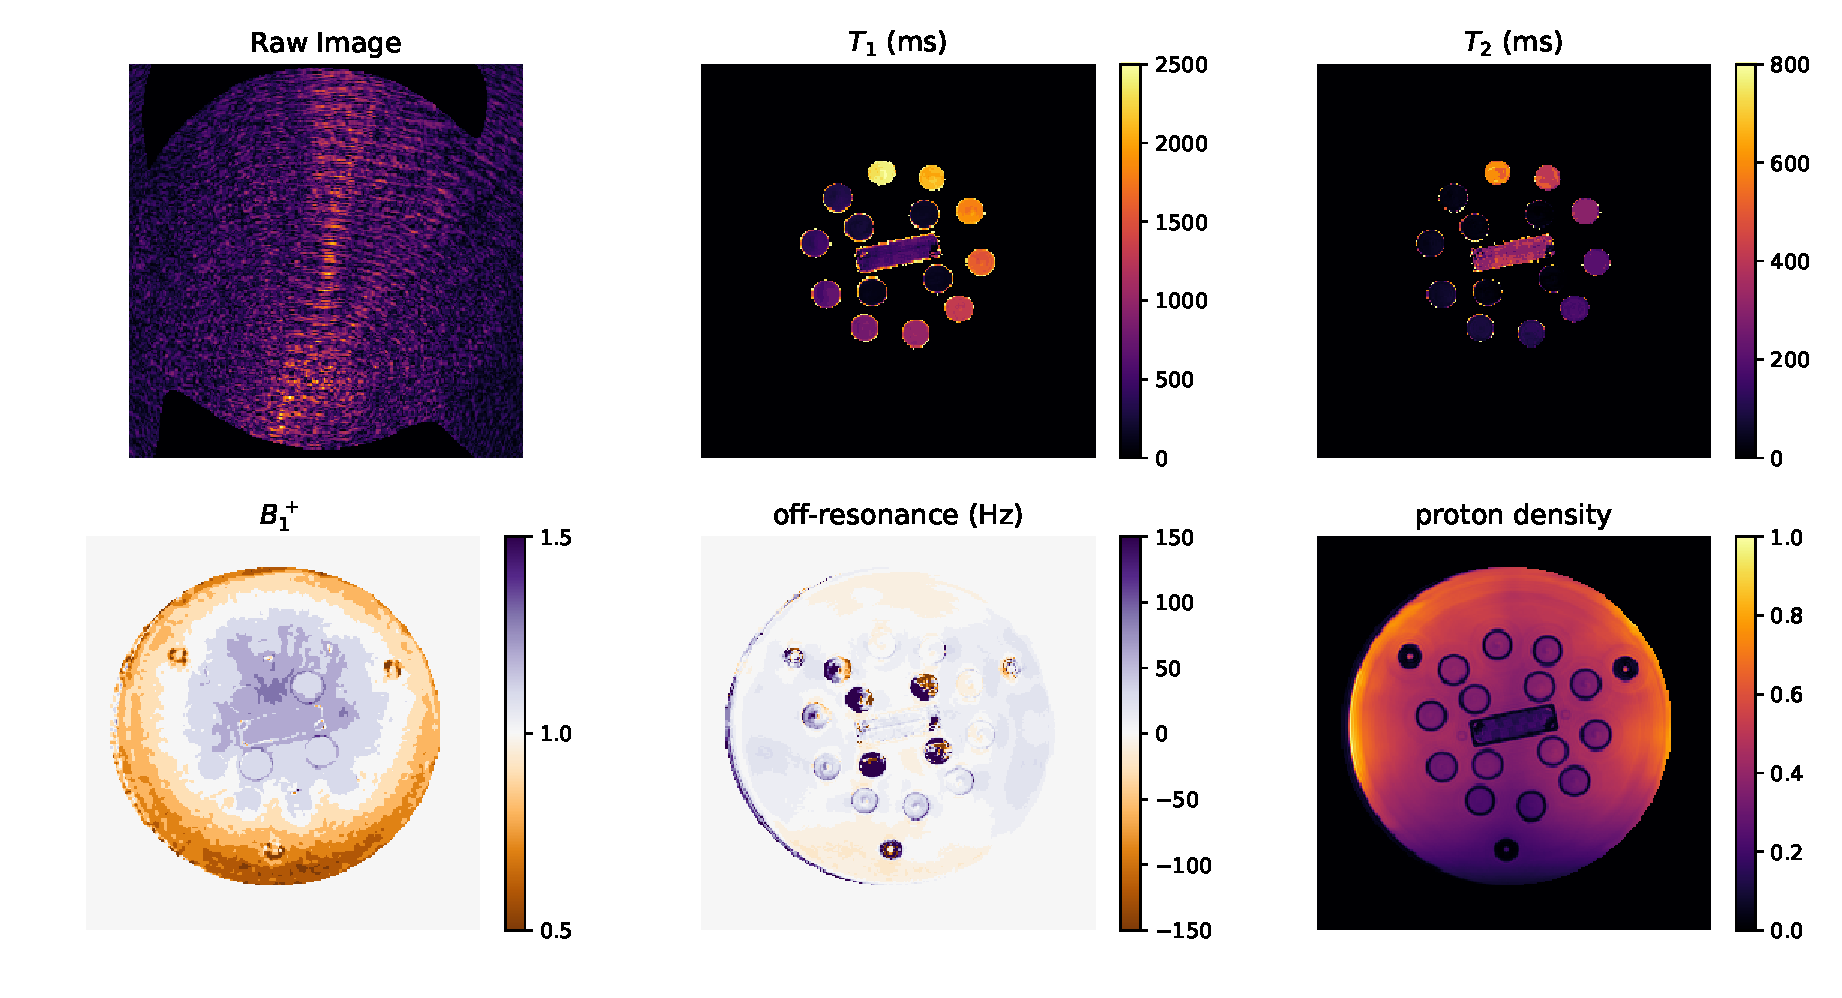
\includegraphics[width=1\textwidth]{../img/intro/mrfmap}
	\end{figure}
\end{frame}

\begin{frame}
\frametitle{研究背景--MRF}
	MRF重建的主要问题:
	\begin{itemize}
		\item 字典生成和模板匹配的速度慢,当字典比较大时,通常需要几十分钟甚至几小时。
		\item 临床中还无法应用,需要快速甚至实时的算法和软件
	\end{itemize}
\end{frame}

%------------------------------------------------
\subsection{主要工作}
\begin{frame}
	\frametitle{主要工作}
	\begin{itemize}
		\item 针对胸部DCE-MRI图像,比较了5中不同的时间方向的稀疏项,并对结果进行了定量分析,确定了适合胸部DCE-MRI的时间稀疏项
		\item 针对胸部DCE-MRI图像,利用提出了基于二阶TGV和核范数的稀疏低秩分解模型
		\item 针对MRF中字典生成和匹配速度慢的问题,开发了一款基于图形处理单元(GPU)的开源软件snapMRF
	\end{itemize}
\end{frame}

\begin{frame}
	\frametitle{发表的论文}
	\begin{itemize}
		\item Dong Wang, Lori R. Arlinghaus, Thomas E. Yankeelov, Xiaoping Yang, and David S. Smith. Quantitative Evaluation of Temporal Regularizers in Compressed Sensing Dynamic Contrast Enhanced MRI of the Breast. (EI,接收)
		\item Dong Wang, Jason Ostenson, and David S. Smith. snapMRF: GPU-Accelerated Magnetic Resonance Fingerprinting Dictionary Generation and Matching using Extended Phase Graphs. (SCI三区,重投)
		\item Dong Wang and Xiaoping Yang. Compressed sensing based DCE-MRI of the breast reconstruction using low rank and sparse decomposition. (在写)
	\end{itemize}
\end{frame}

\begin{frame}
	\frametitle{发表的会议}
	\begin{itemize}
		\item Dong Wang, Lori R. Arlinghaus, Thomas E. Yankeelov, Xiaoping Yang, and David S. Smith. Quantitative Evaluation of Temporal Regularizers in Compressed Sensing Dynamic Contrast Enhanced MRI of the Breast.(ISMRM,2017)
	\end{itemize}
\end{frame}



%------------------------------------------------
\section{胸部DCE-MRI图像压缩感知的时间稀疏正则项的量化评估}
%------------------------------------------------
\AtBeginSection[]
{
    \begin{frame}
        \tableofcontents[currentsection,hideallsubsections]
    \end{frame}
}

\subsection{时间稀疏项}
\begin{frame}
	\frametitle{时间稀疏项}
	\begin{itemize}
		\item 磁共振动态对比增强(DCE-MRI)是通过测量注入造影剂期间和之后的信号,使得图像的每个体素产生一个时间强度曲线,用于定量地估计生理参数,如例如体积转移常数 ($K^{trans}$) 和血管外细胞体积分数 ($v_e$) 等
		\item 这些生理参数有助于给医生提供客观的标准,用于诊断和治疗
		\item 对于胸部DCE-MRI,体素的时间强度曲线决定了参数估计的准确性,高时间分辨率有利于提精确地定量分析
	\end{itemize}
\end{frame}

\begin{frame}
	\frametitle{时间稀疏项}
	\begin{itemize}
		\item 虽然压缩感知已经应用于胸部DCE-MRI中,但目前还没有研究通过量化分析的方式来比较时间方向的稀疏项在DCE-MRI中的表现
		\item 因此对于定量胸部DCE-MRI,不同时间方向的稀疏项对重建误差的影响是未知的
	\end{itemize}
\end{frame}

\begin{frame}
	\frametitle{时间稀疏项}
	本文通过量化分析的方式比较和评估5种不同的时间方向的稀疏项$T$:
\begin{enumerate}
	\item 傅里叶变换的$l_1$范数 ($l_1$-norm of the Fourier transform, FT),
	\item 希尔小波变换的$l_1$范数 ($l_1$-norm of the Haar Wavelet transform, WT),
	\item 全变差 (Total Variation, TV)
	\item 二阶TGV (Second Order TGV, $\texttt{TGV}_{\alpha}^2$),
	\item 核范数 (Nuclear Norm, NN)。
\end{enumerate}
\end{frame}

\begin{frame}
	\frametitle{时间稀疏项}
	\begin{itemize}
		\item 图像大小$192\times 128\times 105$
		\item 采样模式为200个不同的Cartesian采样
		\item 使用FISTA求解
		\item 评价标准为图像的增强信噪比(SER)和肿瘤区域参数的一致性相关系数(CCC)
	\end{itemize}
\end{frame}

\begin{frame}
在每一帧图像上,我们对低频区域进行全采样,对高频区域进行随机采样。
\begin{figure}
\centering
  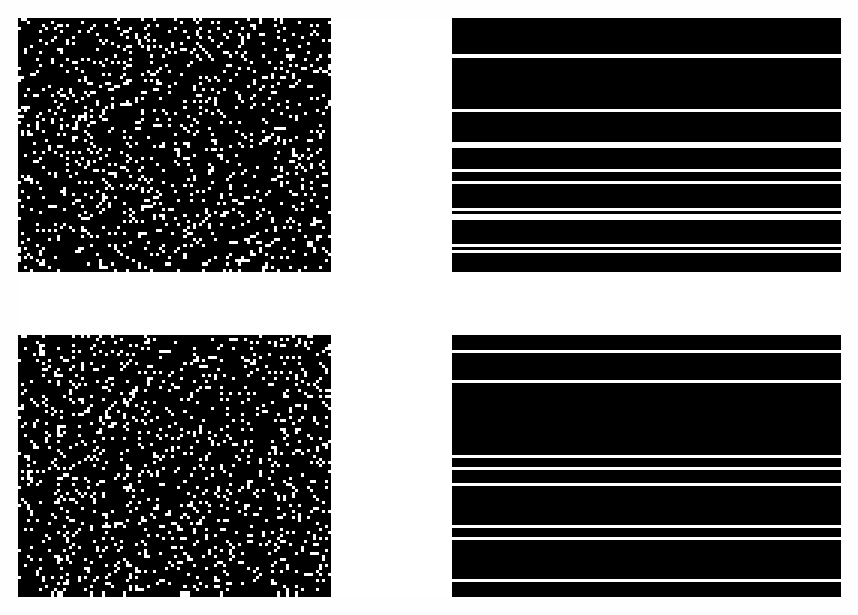
\includegraphics[width=0.6\textwidth]{../img/qetsr/figure1.eps}
\caption{
Cartesian采样模式的例子
}
\end{figure}
\end{frame}

%------------------------------------------------
\subsection{实验结果}
\begin{frame}
\frametitle{实验结果}
NN得到了最高的SER,而TV/TGV$_\alpha^2$得到了最高的CCC,即它们在肿瘤区域的重建效果最好。
\begin{table}
\caption{200个Cartesian采样模式重建的均值SER与CCC}
\centering
\begin{tabular}{lccc}
\hline
稀疏项&SER(dB)&\ccckt&\cccve\\
\hline
Zerofilled & 15.1 & 0.694 & 0.636\\
\hline
FT & 26.4 & 0.763 & 0.575\\
\hline
WT & 21.8 & 0.878 & 0.733\\
\hline
TV & 27.7 & \textbf{0.974} & 0.916\\
\hline
TGV$_\alpha^2$ & 27.8 & \textbf{0.974} & \textbf{0.917}\\
\hline
NN & \textbf{29.1} & 0.842 & 0.799\\

\hline
\end{tabular}
\label{tab:result}
\end{table}
\end{frame}

\begin{frame}
	\frametitle{实验结果}
	\begin{figure}[htbp]
\centerline{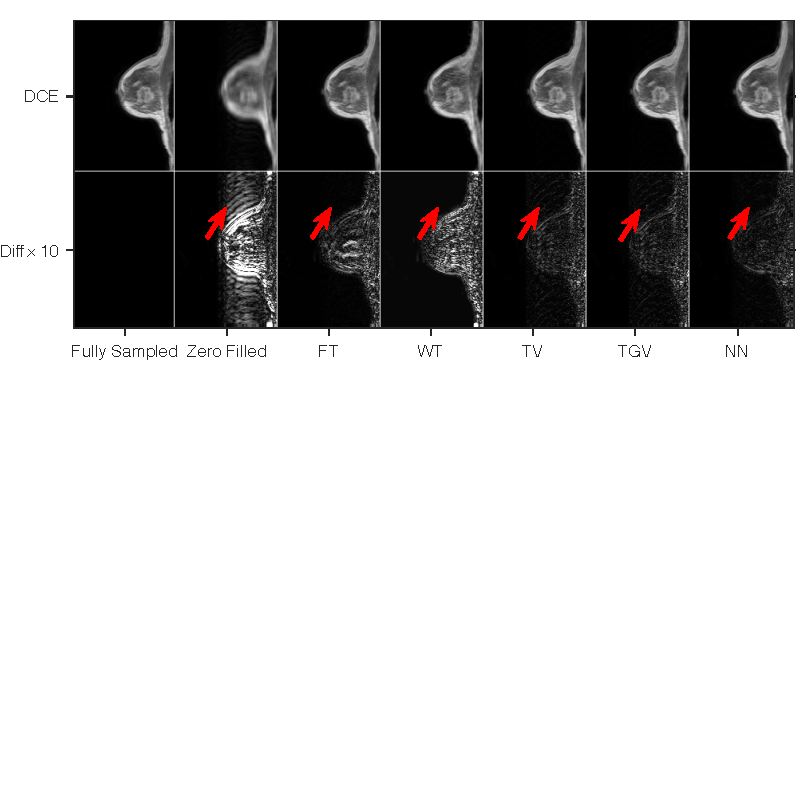
\includegraphics[width=1\textwidth]{../img/qetsr/figure2_1}}
\caption{
第一个Cartesian采样模式下第105帧的重建结果。图中的红色的箭头显示,在视觉上,NN去除背景伪影方面表现最好。
}
\end{figure}
\end{frame}

\begin{frame}
	\frametitle{实验结果}
	\begin{figure}[htbp]
\centerline{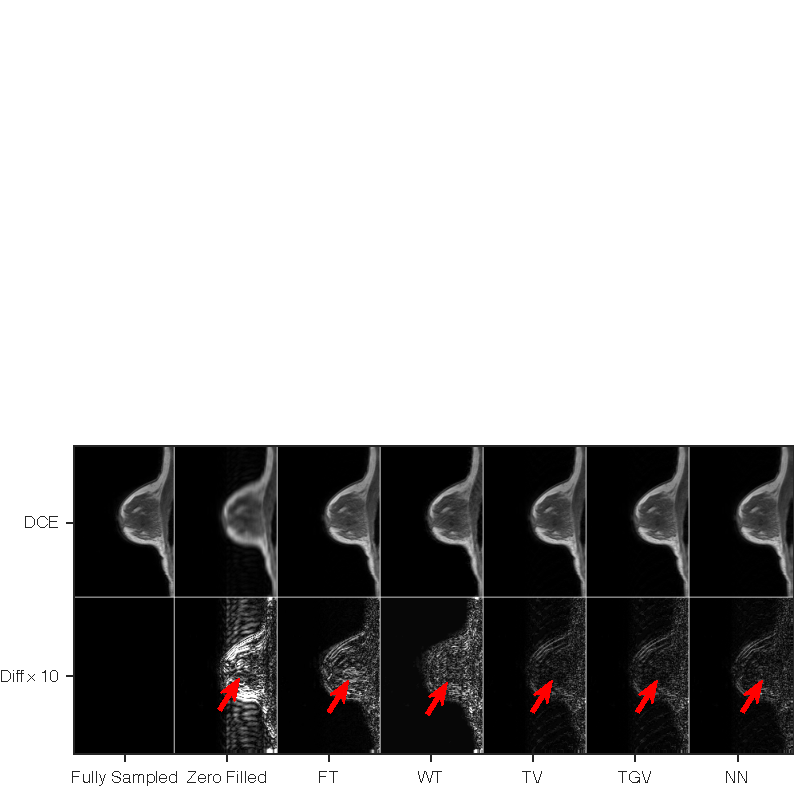
\includegraphics[width=1\textwidth]{../img/qetsr/figure2_2}}
\caption{
第一个Cartesian采样模式下第1帧的重建结果。图中的红色的箭头显示,在视觉上,TV和TGV$_\alpha^2$模型重建肿瘤的效果是最好的。
}
\end{figure}
\end{frame}

\begin{frame}
	\frametitle{实验结果}
	\begin{figure}[htbp]
\centerline{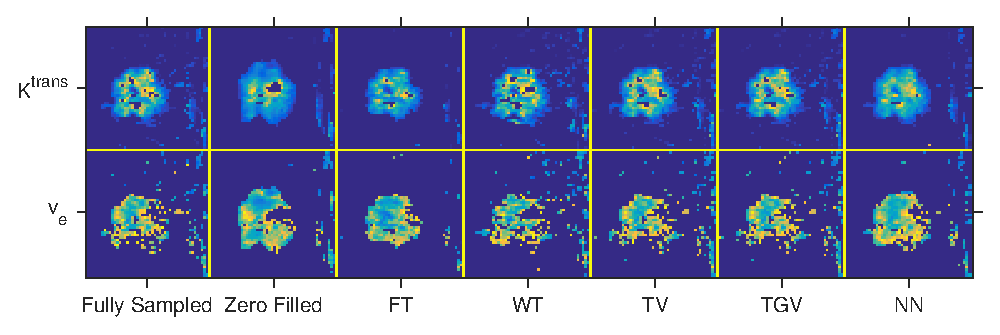
\includegraphics[width=1\textwidth]{../img/qetsr/figure4.eps}}
\caption{
\kt 和\Ve 参数肿瘤部分放大后的图像。在视觉上,TV和TGV$_{\alpha}^2$与全采样的参数图像最接近。
}
\end{figure}
\end{frame}

\begin{frame}
	\frametitle{实验结果}
	\begin{figure}[htbp]
\centerline{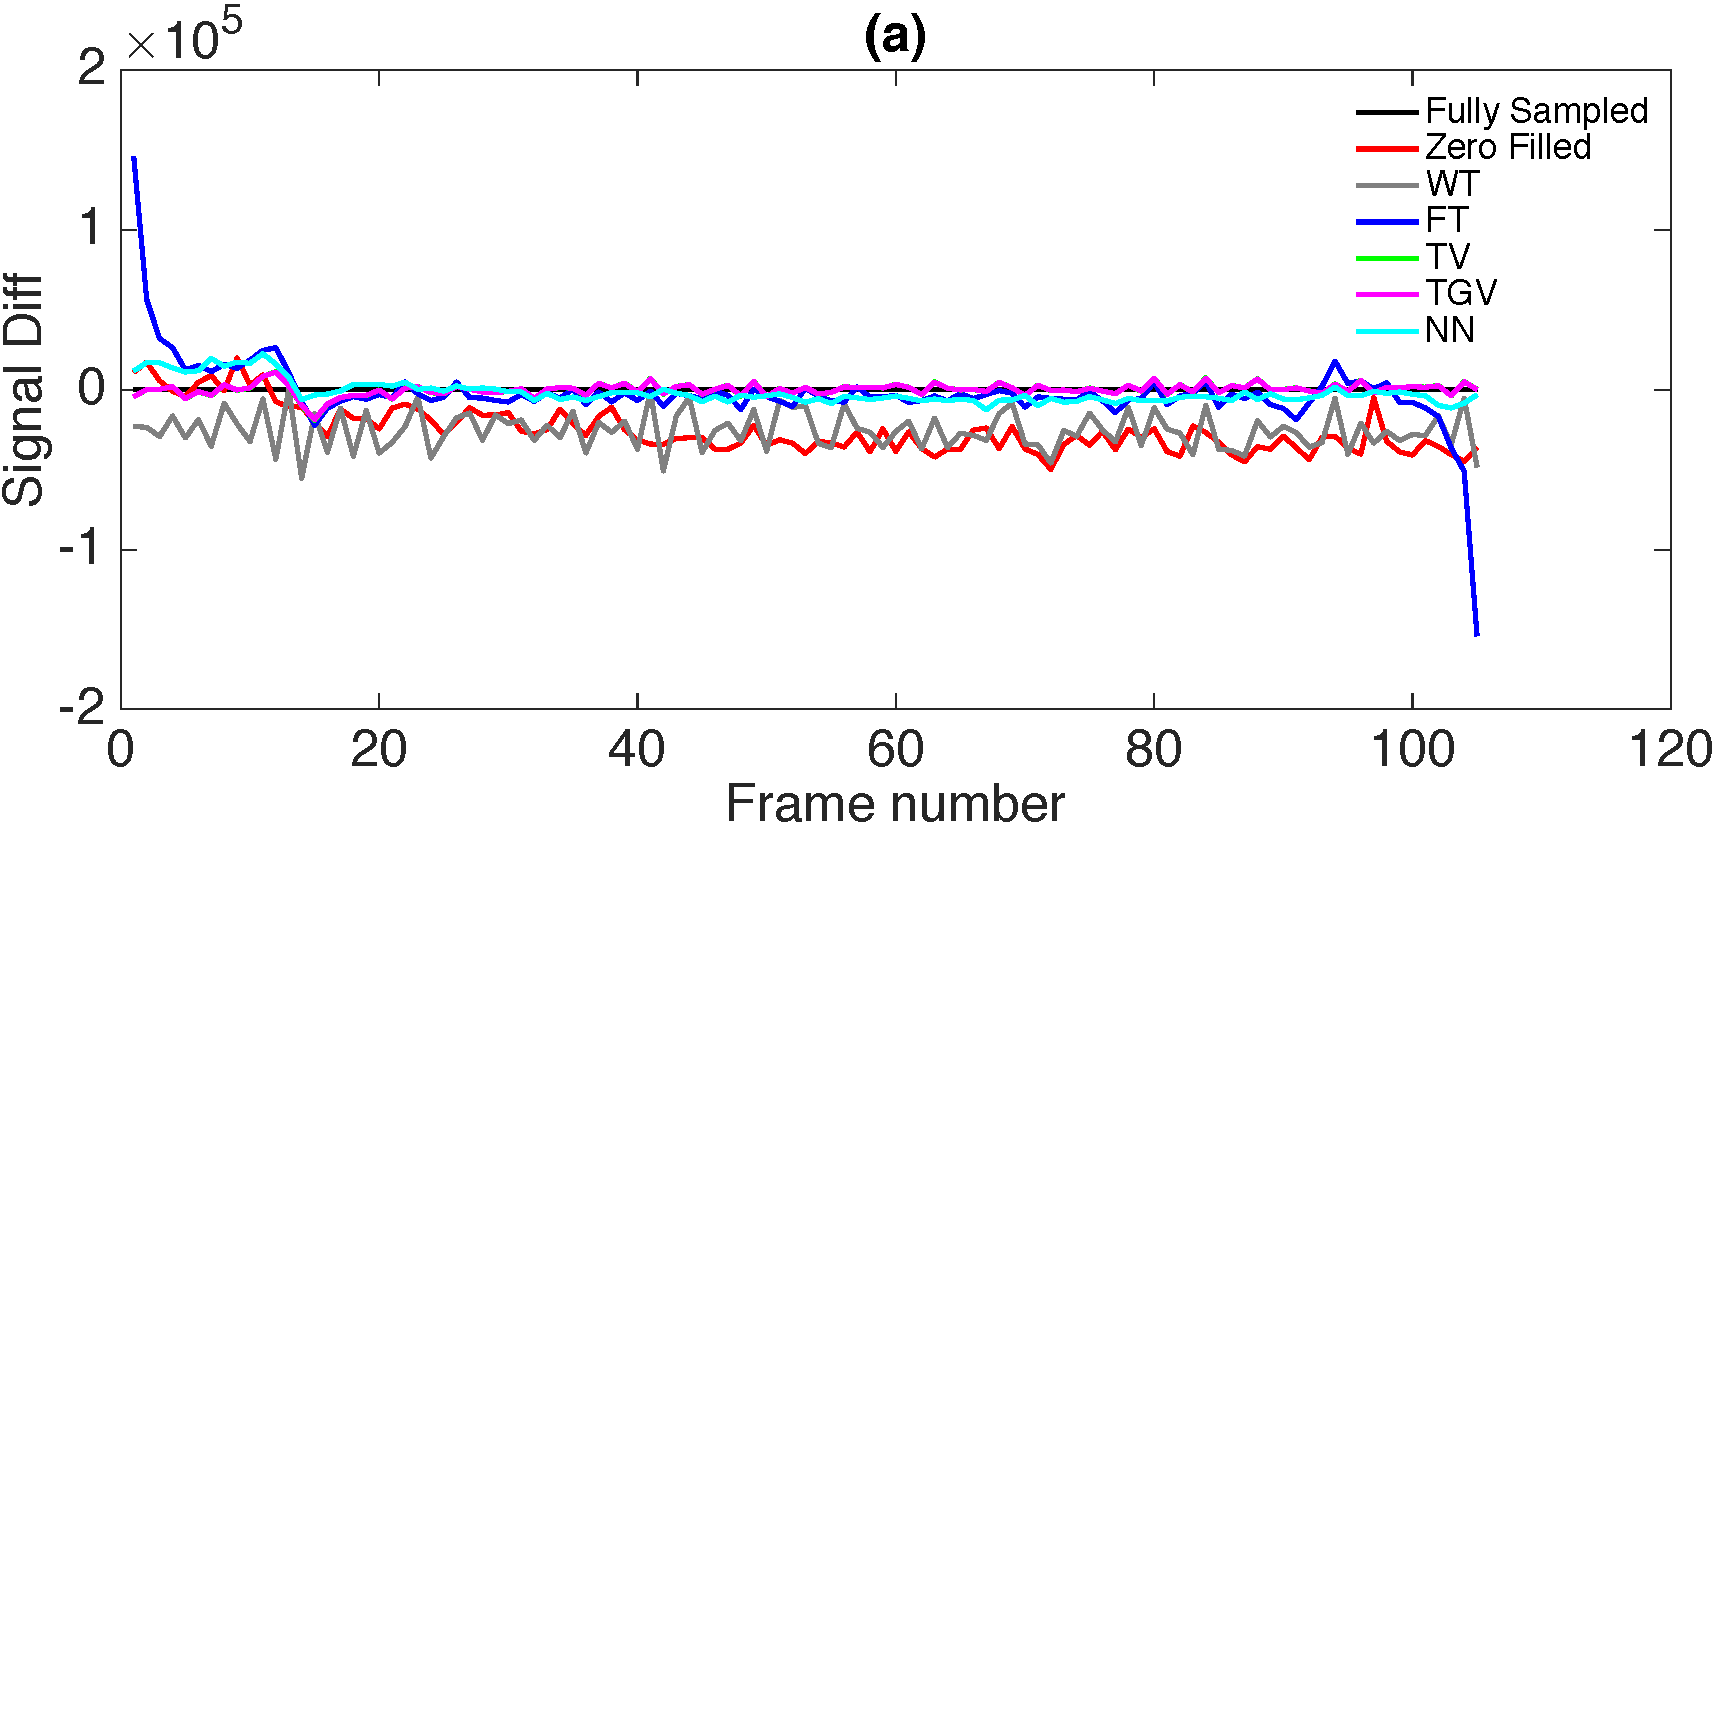
\includegraphics[width=1\textwidth]{../img/qetsr/figure6.pdf}}
\caption{
全采样图像与重建图像肿瘤区域像素时间曲线的比较图。
}
\end{figure}
\end{frame}

%------------------------------------------------
\section{动态MRI图像的低秩和稀疏分解模型}
%------------------------------------------------
\AtBeginSection[]
{
    \begin{frame}
        \tableofcontents[currentsection,hideallsubsections]
    \end{frame}
}

\subsection{基于TGV$_\alpha^2$与核范数的压缩感知重建模型}
\begin{frame}
	\frametitle{基于TGV$_\alpha^2$与核范数的压缩感知重建模型}
	\begin{itemize}
		\item DCE-MRI图像中最重要的问题是时间分辨率和空间分辨率之间的权衡
		\item 高时间分辨率可以提高参数定量分析的准确性
		\item 高空间分辨率有助于提高医生的临床阅读
	\end{itemize}
\end{frame}

\begin{frame}
	\frametitle{基于TGV$_\alpha^2$与核范数的压缩感知重建模型}
	目前基于压缩感知模型的动态MR图像重建有两大类:
	\begin{itemize}
		\item L\&S:旨在寻找一个即低秩又稀疏的解		
	\end{itemize}
	k-t SLR:
		\begin{equation}
	\min_X \frac{1}{2}||AX-B||^2_F+\alpha\|X\|_{\mathrm{TV}}+\beta||X||_*
	\end{equation}
	这里$\|\cdot\|_*$是矩阵的核范数,即矩阵的奇异值的和,而$\|X\|_{\mathrm{TV}}$定义为:
\begin{equation*}
\|\cdot\|_\mathrm{TV} = \sqrt{(\nabla_x \cdot)^2 + (\nabla_y \cdot)^2+(\nabla_t \cdot)^2},
\end{equation*}
其中$\nabla_x$,$\nabla_y$和$\nabla_t$分别为$x$,$y$和$t$方向上的梯度算子。\\
	问题:TV正则项导致阶梯效应,并且重建图像的边界模糊。	
\end{frame}

\begin{frame}
	\frametitle{基于TGV$_\alpha^2$与核范数的压缩感知重建模型}
	\begin{itemize}
	\item L+S:将动态图像分解为两个部分,低秩部分和稀疏部分。其中低秩部分用来建模时间上高度相关的背景,稀疏部分用来建模背景之上的动态信息。
    \end{itemize}
		TTV+NN:
		\begin{equation}
	\min_{L,S}\frac{1}{2}||A(L+S)-B||_F^2 + \alpha||\nabla_tS||_1 + \beta\|L\|_*
	\end{equation}	
	问题:模型只用到了时间方向的稀疏项,重建模型的空间分辨率低。
\end{frame}

\begin{frame}
	\frametitle{基于TGV$_\alpha^2$与核范数的压缩感知重建模型}
	Bredies提出了基于图像高阶信息的Total Generalized Variation (TGV)的理论框架。TGV$_\alpha^2$可很好地刻画图像中的平滑部分,在抑制阶梯效应方面有着良好的表现。
	
	针对TV正则项导致阶梯效应的问题,并且利用图像分解的思想,我们提出了基于$TGV_\alpha^2$和核范数的L+S模型:
	\begin{equation}
	\min_{L,S}\frac{1}{2}||A(L+S)-B||_2^2 + \mathrm{TGV}_\alpha^2(S) + \beta\|L\|_*
	\label{equ:tgvlr}
\end{equation}
\end{frame}

\begin{frame}
	\frametitle{基于TGV$_\alpha^2$与核范数的压缩感知重建模型}
	\begin{itemize}
		\item 三组数据,体模、心脏灌注和胸部DCE-MRI
		\item 采样模式为伪径向采样,在每一帧上均匀选取32条采样线
		\item 使用Primal-Dual求解
		\item 评价标准为SER和结构相似性测度(SSIM)
	\end{itemize}
\end{frame}

%------------------------------------------------
\subsection{实验结果}
\begin{frame}
	\frametitle{基于TGV$_\alpha^2$与核范数的压缩感知重建模型}
	\begin{table}
	\center{}
	\caption{伪径向采样模式下不同模型在不同数据上重建结果的比较}
	\begin{tabular}{|c|c|c|c|c|c|}
		\hline
		\multicolumn{2}{|c|}{\diagbox{Models}{Datesets}}& PINCAT & Cardiac & Breast 1 & Breast 2\\	
		\hline
		\multirow{2}{*}{k-t SLR}
		&SER & 31.42 & 18.26 & 26.99 & 25.45\\
		\cline{2-6}&SSIM & \textcolor{red}{0.9935} & 0.9452 & 0.9873 & 0.9627\\
		\hline
		\multirow{2}{*}{TTV+NN}
		&SER & 29.05 & 18.72 & 29.67 & 29.12\\
		\cline{2-6}&SSIM & 0.9617 & 0.9455 & 0.9848 & 0.9697\\
		\hline
		\multirow{2}{*}{Proposed}
		&SER & \textcolor{red}{32.53} & \textcolor{red}{19.72} & \textcolor{red}{30.53} & \textcolor{red}{29.32}\\
		\cline{2-6}&SSIM & 0.9852 & \textcolor{red}{0.9546} & \textcolor{red}{0.9922} & \textcolor{red}{0.9759}\\
		\hline
	\end{tabular}
\end{table}
\end{frame}

\begin{frame}
	\frametitle{基于TGV$_\alpha^2$与核范数的压缩感知重建模型}
	\begin{figure}[htbp]
	\centering
		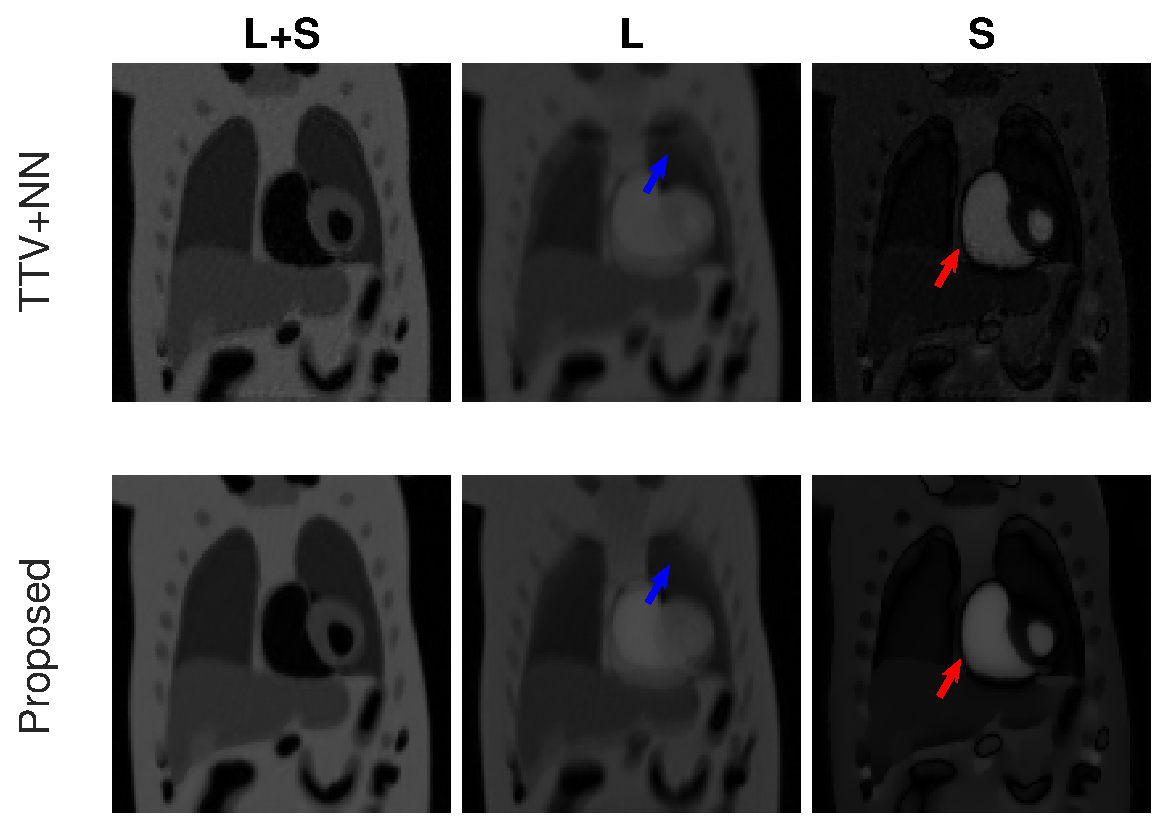
\includegraphics[width=0.8\textwidth]{../img/tgvnn/pincat_1_l+s.eps}
	\caption{L+S模型低秩与稀疏分解效果。PINCAT}
\end{figure}
\end{frame}

\begin{frame}
	\frametitle{基于TGV$_\alpha^2$与核范数的压缩感知重建模型}
	\begin{figure}[htbp]
	\centering
		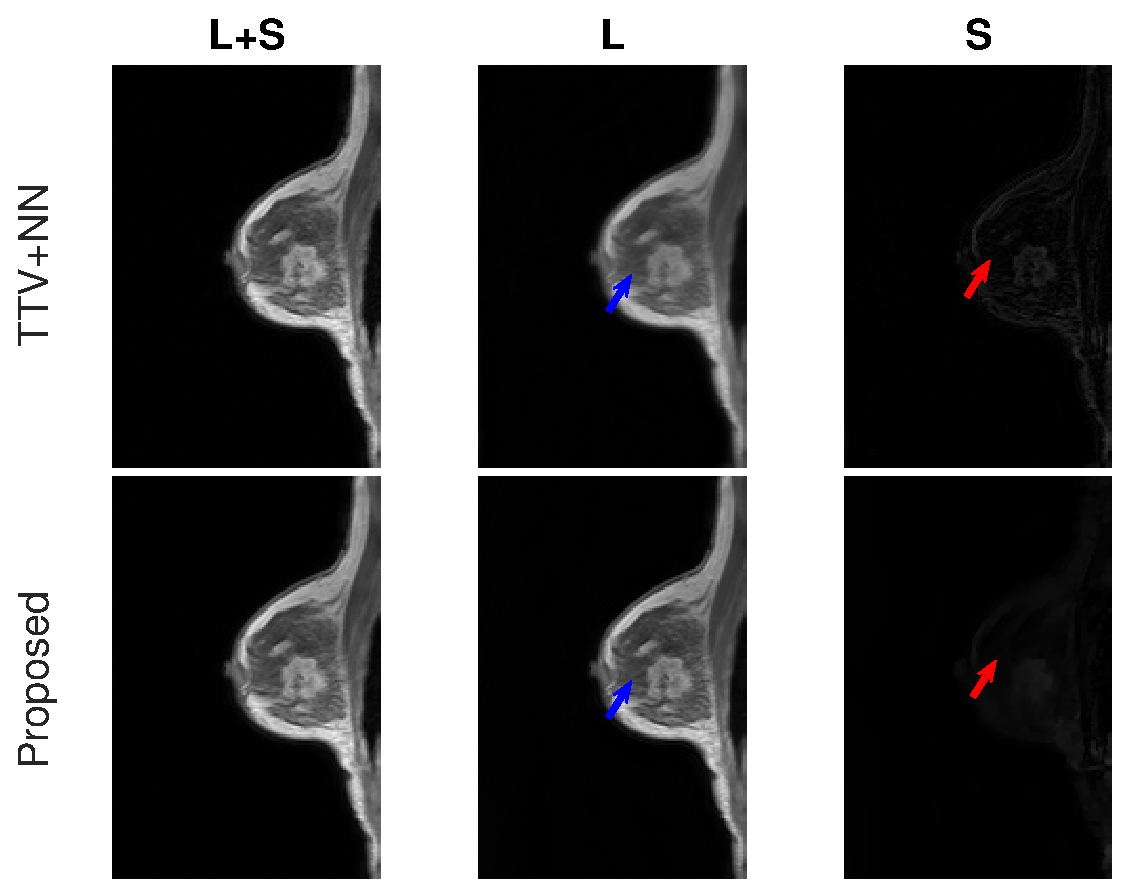
\includegraphics[width=0.8\textwidth]{../img/tgvnn/breast1_55_l+s.eps}
	\caption{L+S模型低秩与稀疏分解效果。Breast}
\end{figure}
\end{frame}

\begin{frame}
	\frametitle{基于TGV$_\alpha^2$与核范数的压缩感知重建模型}
	\begin{figure}[htbp]
	\centering
		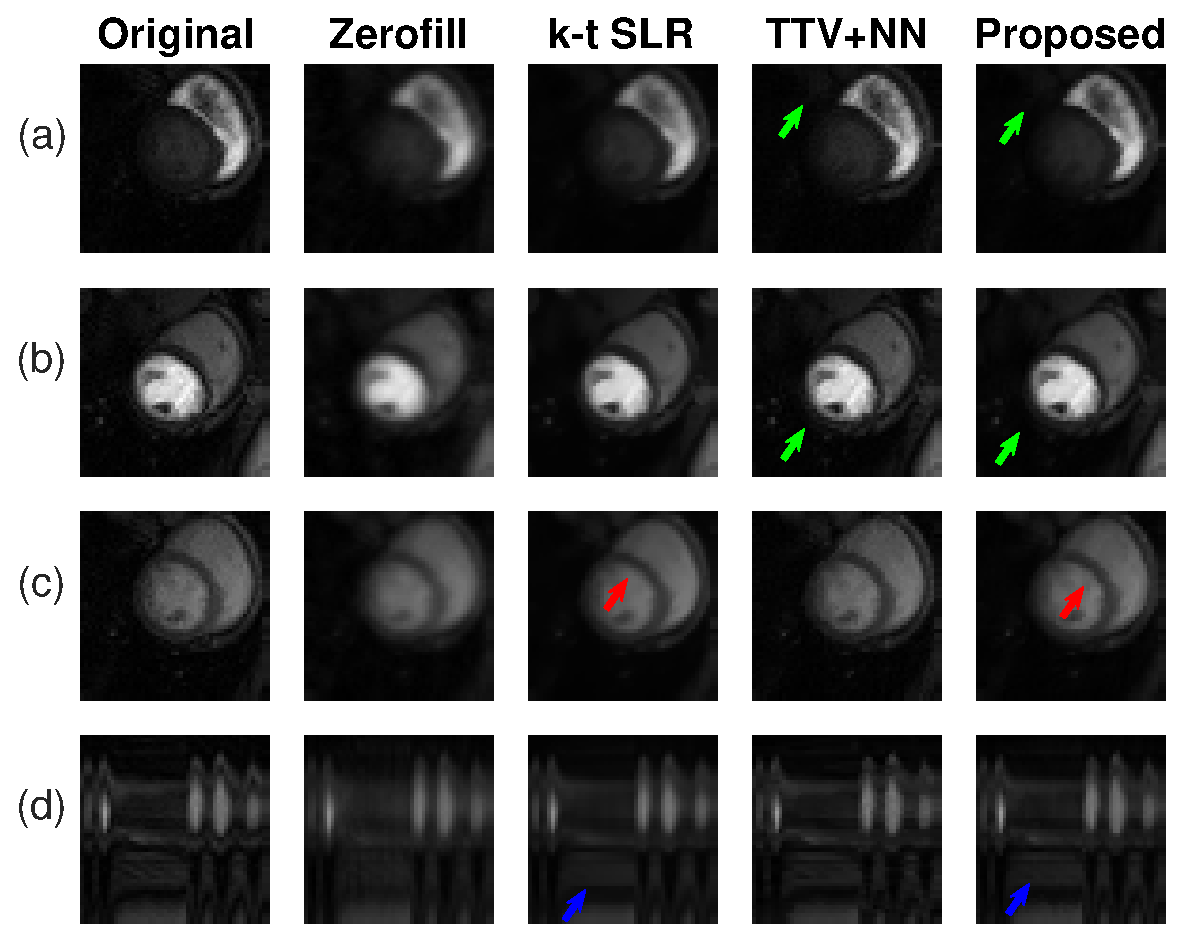
\includegraphics[width=0.8\textwidth]{../img/tgvnn/perfusion_frames.eps}
	\caption{Cartiac重建图像比较。(a)第11帧图像;(b)第21帧图像;(c)第54帧图像。(d)通过心脏中心的一列在时间上的演化图像。}
\end{figure}
\end{frame}

%------------------------------------------------
\section{基于GPU的实时磁共振指纹的字典生成和匹配}
%------------------------------------------------
\AtBeginSection[]
{
    \begin{frame}
        \tableofcontents[currentsection,hideallsubsections]
    \end{frame}
}

\subsection{GPU程序实现}
\begin{frame}
	\frametitle{GPU程序实现}
	\begin{itemize}
		\item MRF重建参数图的过程中需要生成一个包含不同参数的组织随着时间演化的字典,而这个过程十分耗时,尤其是使用扩展相图模型(EPG)进行字典模拟时。
		\item 采集信号后,需要将信号与字典进行匹配,从而重建出参数图。这个过程需要计算向量的内积,当字典个数和指纹体素个数很多时,计算的代价也会很大。
	\end{itemize}	
\end{frame}

\begin{frame}
	\frametitle{GPU程序实现}
	针对MRF重建参数图计算时间长的问题,我们开发了一款开源有效的MRF重建软件snapMRF,用于在GPU上平行计算字典生成和模板匹配。snapMRF的代码结构入下:
	\begin{itemize}
		\item CSV文件中读取MR序列的成像参数
		\item 从命令行读取字典的配置信息($T_1$, $T_2$, $B_0$, $B_1^+$)
		\item 直接在GPU上生成字典
		\item 将指纹体素与字典匹配
		\item 保存结果
	\end{itemize}
\end{frame}

\begin{frame}
	\frametitle{GPU程序实现}
	\begin{itemize}
		\item 我们和另外两款开源的软件进行比较,它们分别是EPG-X(MATLAB, CPU)和PnP-MRF(C, CPU)。
		\item 从运行时间和重建参数质量两方面进行比较
		\item 体模数据和活体人脑数据
	\end{itemize}
\end{frame}

%------------------------------------------------
\subsection{实验结果}
\begin{frame}
	\frametitle{实验结果}
	\begin{figure}[htbp]
	\centering
		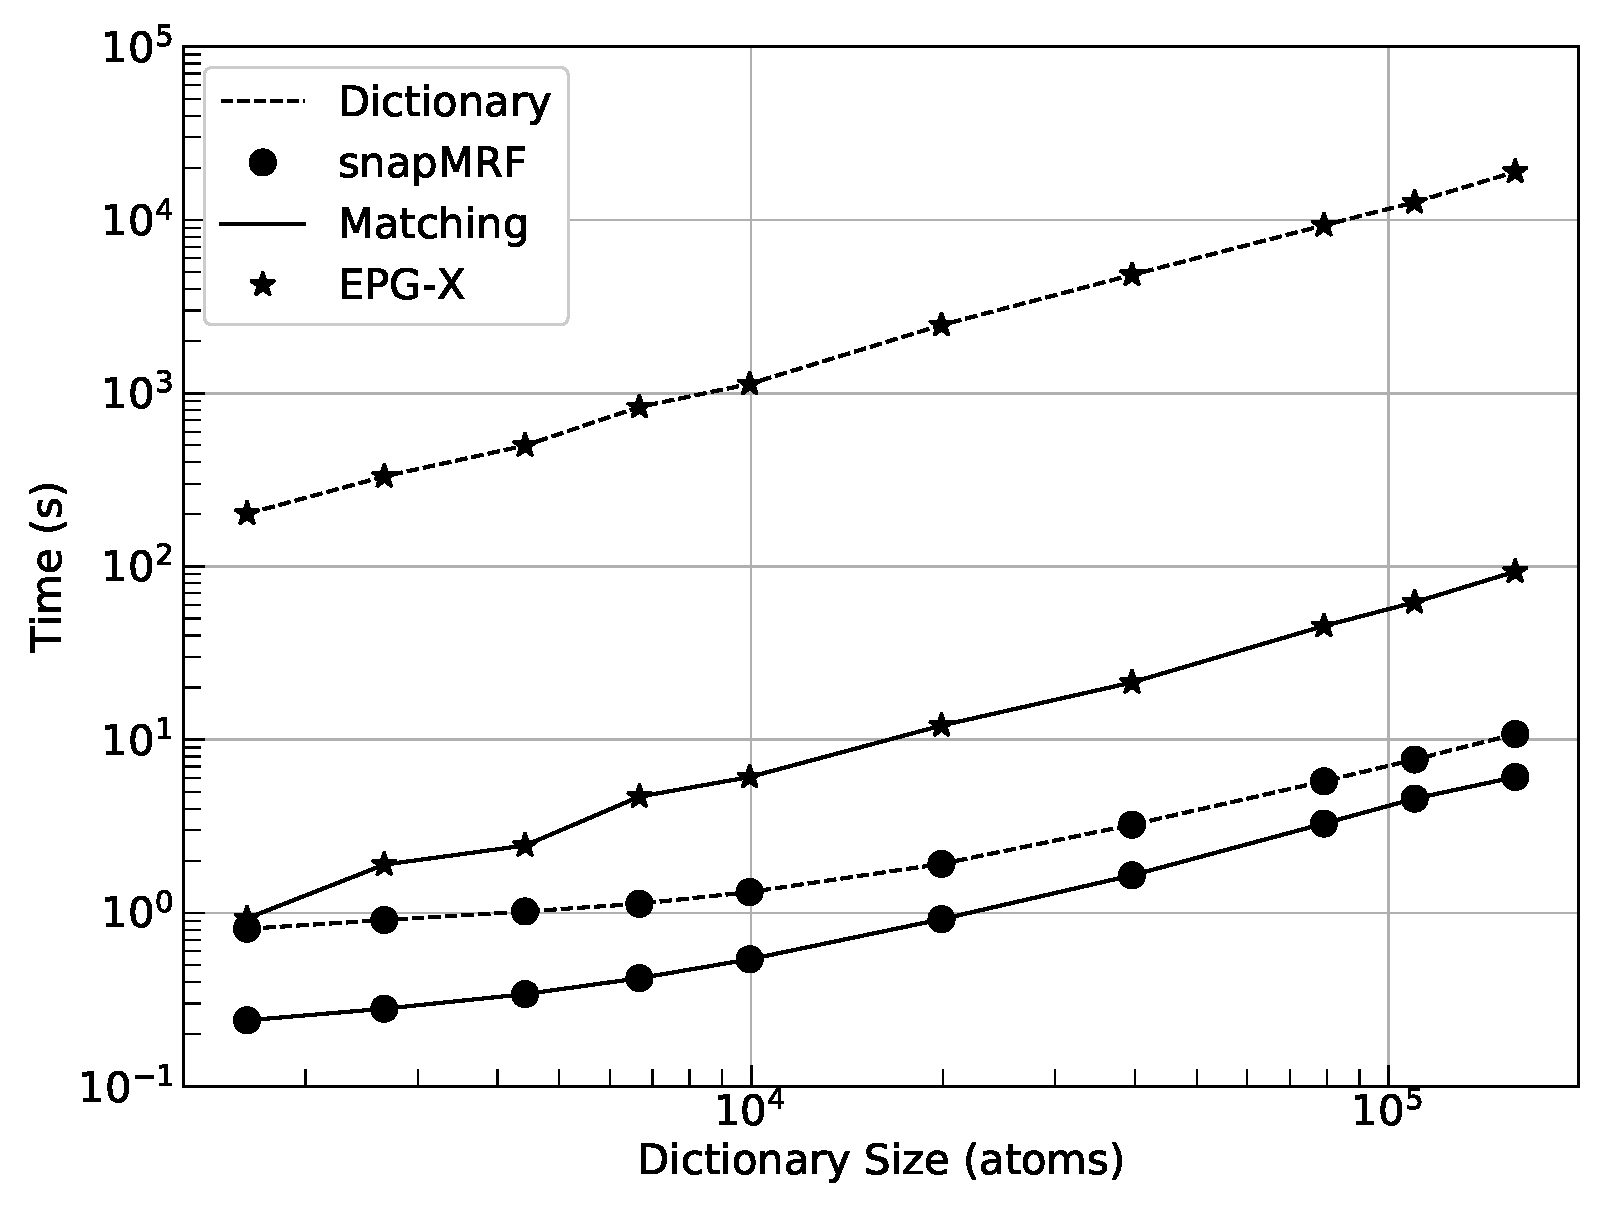
\includegraphics[width=0.7\textwidth]{../img/snapmrf/time_vs_epgx.eps}
	\caption{snapMRF与EPG-X}
\end{figure}
\end{frame}

\begin{frame}
	\frametitle{基于TGV$_\alpha^2$与核范数的压缩感知重建模型}
	\begin{figure}[htbp]
	\centering
		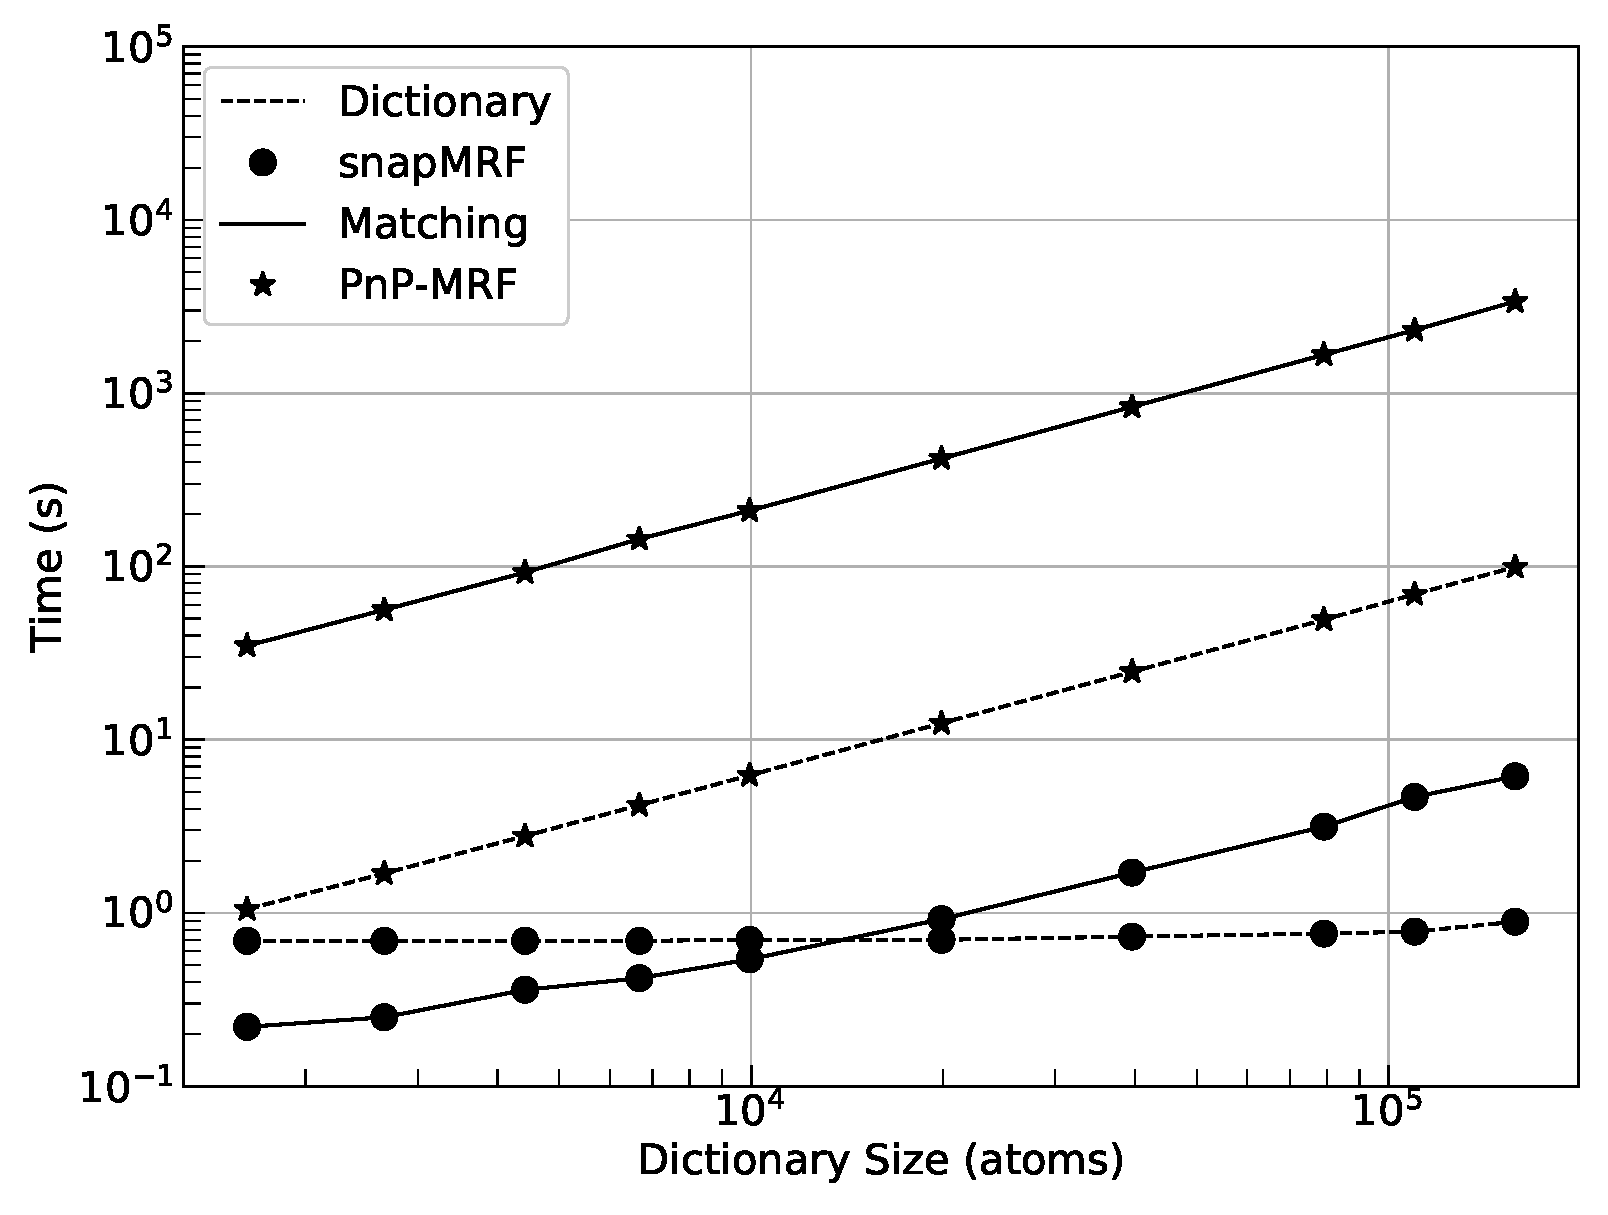
\includegraphics[width=0.7\textwidth]{../img/snapmrf/time_vs_pnp.eps}
	\caption{snapMRF与PnP-MRF}
\end{figure}
\end{frame}

\begin{frame}
\frametitle{实验结果}
	\begin{table}
\caption{snapMRF与EPG-X在字典生成和模板匹配上运行时间的比较。字典大小为100,000,指纹体素个数为240$\times$240。注意snapMRF比EPG-X快很多。}
\centering
\label{tab:time}
\begin{tabular}{rrrrrr}
\specialrule{0em}{3pt}{3pt}
\toprule[2pt]
Running time & EPG-X & snapMRF & snapMRF & snapMRF\\ 
(ms) & fix$T_R$ & fix$T_R$ & var$T_R$ & var$T_R$+$B_1^+$\\
\midrule[1pt]
phantom/dict & 17797.05 & 11.00 & 7.42 & 9.39 \\
phantom/match & 137.13 & 5.97 & 4.14 & 4.88\\
brain/dict & 18629.82 & 11.29 & 7.63 & 8.72 \\
brain/match & 143.55 & 6.13 & 4.23 & 4.63 \\
\bottomrule[2pt]
\end{tabular}
\end{table}
\end{frame}

\begin{frame}
\frametitle{实验结果}
\begin{figure}
 \subfigure[$T_1$精度]{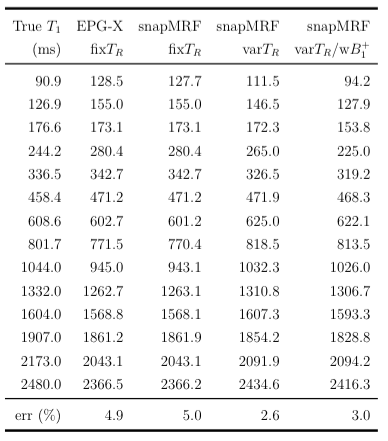
\includegraphics[width=2in]{../img/snapmrf/t1.png}}
 \subfigure[$T_2$精度]{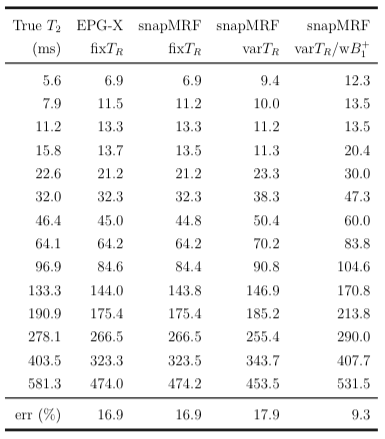
\includegraphics[width=2in]{../img/snapmrf/t2.png}}
\end{figure}
\end{frame}

\begin{frame}
\frametitle{实验结果}
\begin{figure}
\centering
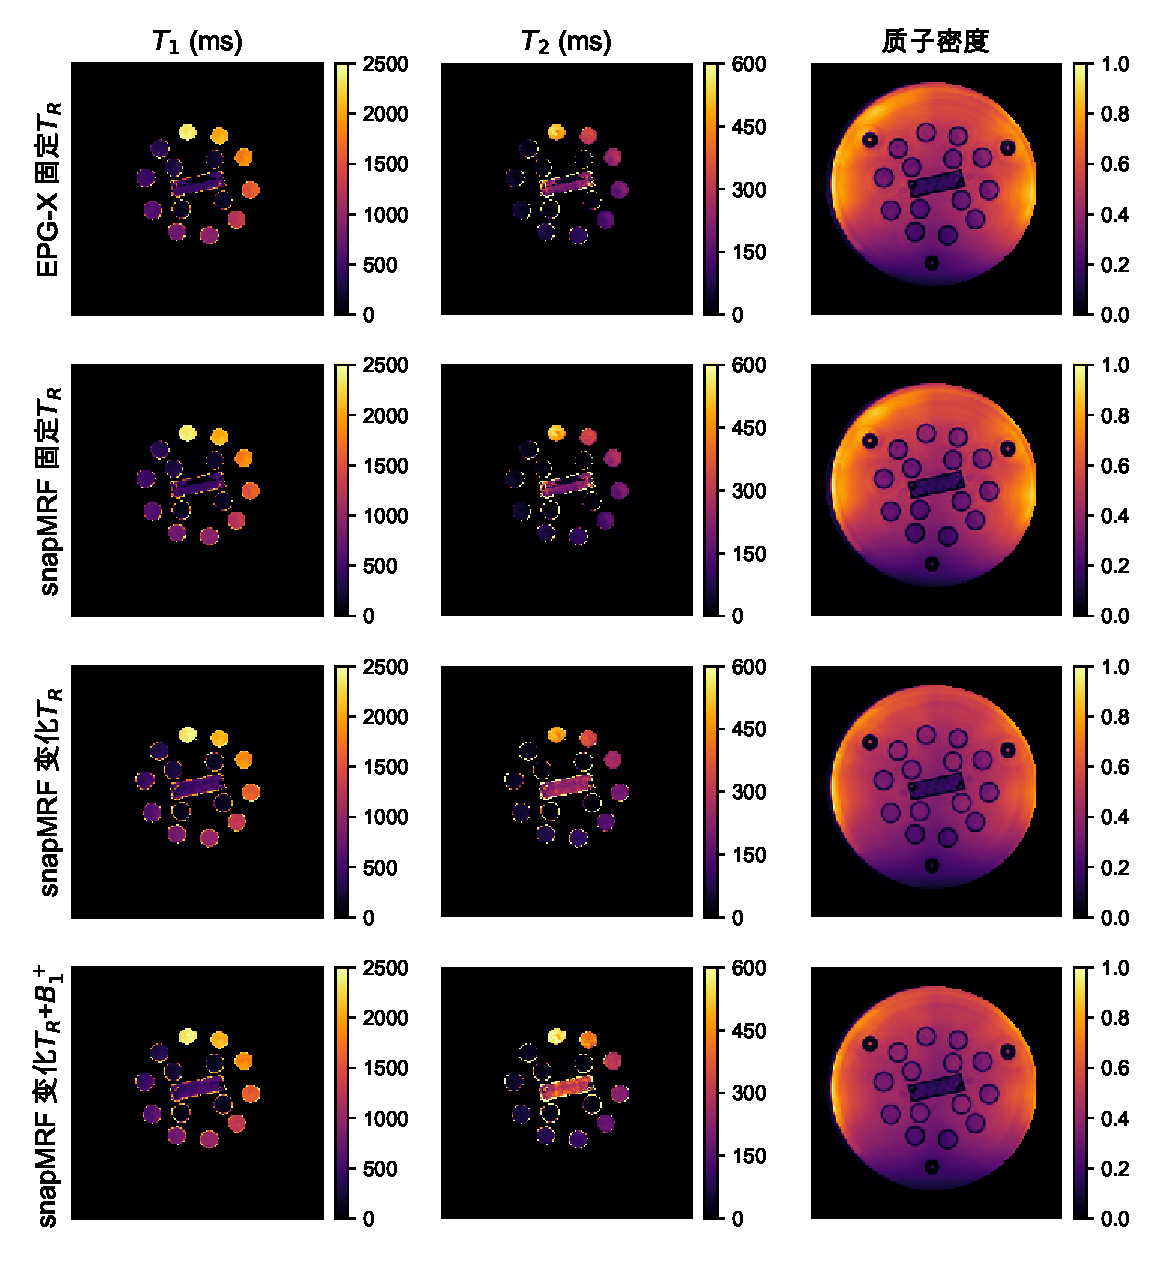
\includegraphics[width=0.6\textwidth]{../img/snapmrf/figure2.eps}
\end{figure}
\end{frame}

\begin{frame}
\frametitle{实验结果}
\begin{figure}
\centering
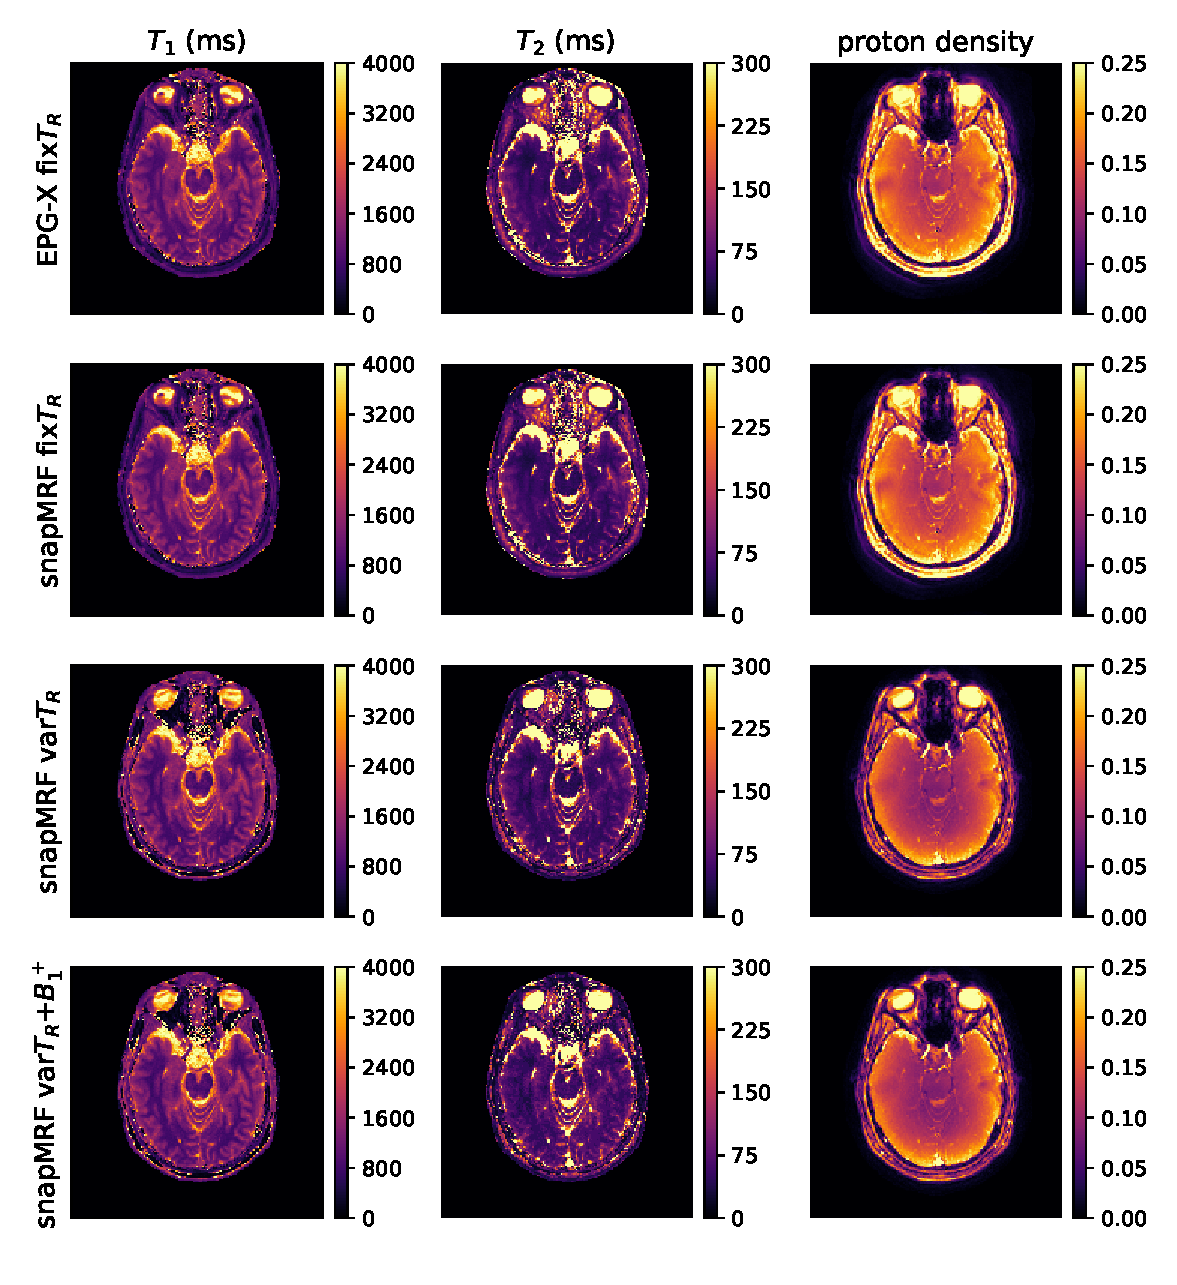
\includegraphics[width=0.6\textwidth]{../img/snapmrf/figure3.eps}
\end{figure}
\end{frame}

%------------------------------------------------

\begin{frame}
\centerline{非常感谢大家来参加我的博士论文学位答辩!}
\centerline{谢谢大家的帮助和指导!}
\end{frame}

%----------------------------------------------------------------------------------------
\end{document}